\documentclass{article}
\usepackage[utf8]{inputenc}
\usepackage[T1]{fontenc}
\usepackage{geometry}
\geometry{margin=1.00in}
\usepackage{hyperref}
\usepackage{xurl}
\usepackage{booktabs}
\usepackage[table]{xcolor}
\usepackage{array}
\usepackage{colortbl}
\usepackage{tikz}
\usetikzlibrary{positioning, shapes.multipart, shapes.geometric, calc, arrows.meta, fit}
\usepackage{enumitem}
\usepackage{verbatim}

\title{System Documentation: Recipe Management Application}
\author{Jaehoon Song} 
\date{\today}

\begin{document}

\maketitle

\section{Introduction}
This document provides the formal specifications for the Recipe and Ingredient management system in accordance with \textbf{ISO/IEC/IEEE 29148:2018} software-requirements practice. It specifies:
\begin{itemize}[noitemsep]
  \item \textbf{Backend services:} HTTP endpoints, validation logic, database integration, and response contracts (Javalin REST API).
  \item \textbf{Client application:} Multi-page web UI requirements expressed through UML use-case models, navigation maps, UI element inventories, and interaction (sequence) diagrams.
\end{itemize}
The system enables user registration and authentication, recipe CRUD and search for all authenticated chefs, and admin-only ingredient taxonomy management.

\subsection{Architecture}
The system is built utilizing a robust \textbf{3-Layer Architecture}, leveraging the \textbf{Javalin Framework} for HTTP routing and handling:
\begin{itemize}
    \item \textbf{Controller Layer:} Manages all incoming HTTP requests via Javalin handlers (e.g., \texttt{RecipeController}, \texttt{AuthenticationController}). It extracts path/query parameters and request bodies, interacts with the Service Layer, and responds with appropriate JSON structures and HTTP status codes.
    \item \textbf{Service Layer:} Encapsulates all business logic and validation rules (e.g., \texttt{RecipeService}). It acts as the intermediary between the controllers and DAOs, ensuring data integrity.
    \item \textbf{Data Access Object (DAO) Layer:} Abstracts all direct database interactions using JDBC. It executes CRUD operations against the in-memory H2 database using \texttt{ConnectionUtil}.
\end{itemize}

\newpage

\subsection{Database Entities}
Figure~\ref{fig:uml-erd} shows a compact \textbf{Crow's Foot} (IE) style ERD for the primary tables. 

\begin{figure}[htbp]
\centering
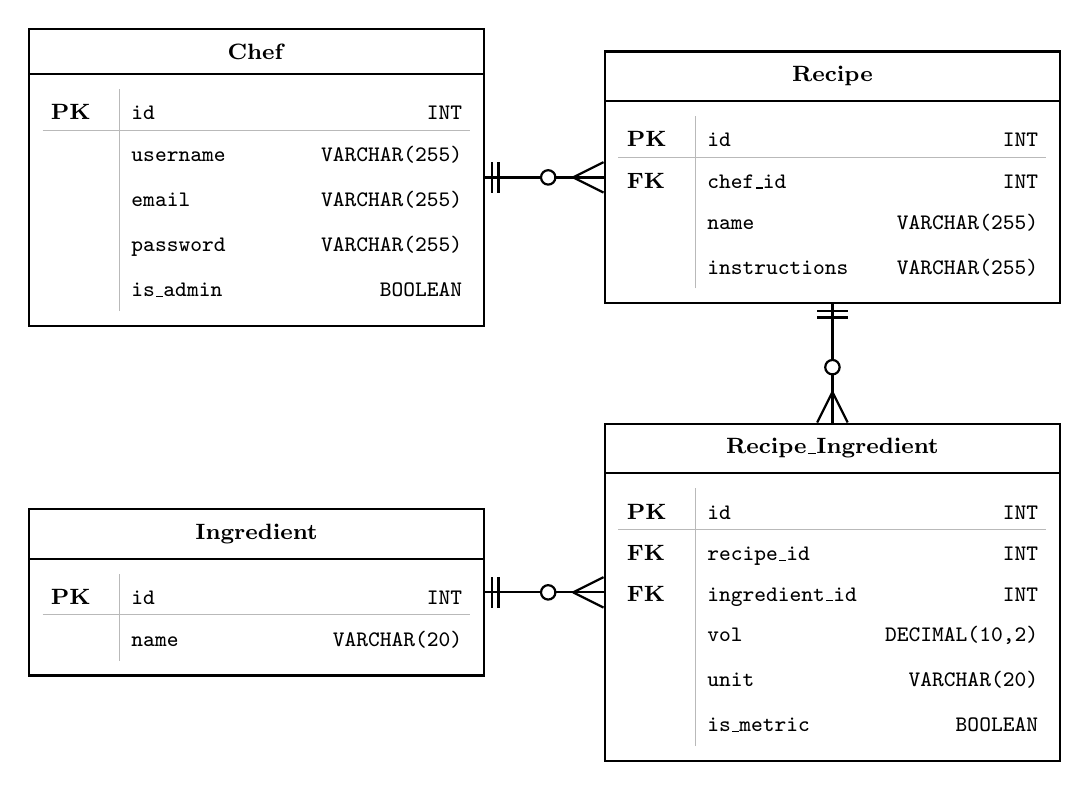
\begin{tikzpicture}[
  font=\footnotesize,
  entity/.style={
    rectangle split,
    rectangle split parts=2,
    draw,
    thick,
    minimum width=5.5cm,
    inner sep=5pt,
    rectangle split part align={center, left},
  },
]
% --- Chef ---
\node[entity] (Chef) {
  \textbf{Chef}
  \nodepart{two}
  {\setlength{\tabcolsep}{2pt}%
   \setlength{\extrarowheight}{2.5pt}%
   \renewcommand{\arraystretch}{1.22}%
   \begin{tabular}{@{\hspace{3pt}}p{8mm}!{\color{gray!55}\vrule width 0.35pt}@{\hspace{4pt}}p{4.2cm}@{\hspace{3pt}}}
  \textbf{PK} & \texttt{id}\hfill\texttt{INT}\\
  \arrayrulecolor{gray!55}\hline\arrayrulecolor{black}
   & \texttt{username}\hfill\texttt{VARCHAR(255)}\\
   & \texttt{email}\hfill\texttt{VARCHAR(255)}\\
   & \texttt{password}\hfill\texttt{VARCHAR(255)}\\
   & \texttt{is\_admin}\hfill\texttt{BOOLEAN}\\
  \end{tabular}%
  }
};

% --- Recipe ---
\node[entity, right=1.5cm of Chef] (Recipe) {
  \textbf{Recipe}
  \nodepart{two}
  {\setlength{\tabcolsep}{2pt}%
   \setlength{\extrarowheight}{2.5pt}%
   \renewcommand{\arraystretch}{1.22}%
   \begin{tabular}{@{\hspace{3pt}}p{8mm}!{\color{gray!55}\vrule width 0.35pt}@{\hspace{4pt}}p{4.2cm}@{\hspace{3pt}}}
  \textbf{PK} & \texttt{id}\hfill\texttt{INT}\\
  \arrayrulecolor{gray!55}\hline\arrayrulecolor{black}
  \textbf{FK} & \texttt{chef\_id}\hfill\texttt{INT}\\
   & \texttt{name}\hfill\texttt{VARCHAR(255)}\\
   & \texttt{instructions}\hfill\texttt{VARCHAR(255)}\\
  \end{tabular}%
  }
};

% --- Recipe_Ingredient ---
\node[entity, below=1.5cm of Recipe] (RecipeIngredient) {
  \textbf{Recipe\_Ingredient}
  \nodepart{two}
  {\setlength{\tabcolsep}{2pt}%
   \setlength{\extrarowheight}{2.5pt}%
   \renewcommand{\arraystretch}{1.22}%
   \begin{tabular}{@{\hspace{3pt}}p{8mm}!{\color{gray!55}\vrule width 0.35pt}@{\hspace{4pt}}p{4.2cm}@{\hspace{3pt}}}
  \textbf{PK} & \texttt{id}\hfill\texttt{INT}\\
  \arrayrulecolor{gray!55}\hline\arrayrulecolor{black}
  \textbf{FK} & \texttt{recipe\_id}\hfill\texttt{INT}\\
  \textbf{FK} & \texttt{ingredient\_id}\hfill\texttt{INT}\\
   & \texttt{vol}\hfill\texttt{DECIMAL(10,2)}\\
   & \texttt{unit}\hfill\texttt{VARCHAR(20)}\\
   & \texttt{is\_metric}\hfill\texttt{BOOLEAN}\\
  \end{tabular}%
  }
};

% --- Ingredient ---
\node[entity, left=1.5cm of RecipeIngredient] (Ingredient) {
  \textbf{Ingredient}
  \nodepart{two}
  {\setlength{\tabcolsep}{2pt}%
   \setlength{\extrarowheight}{2.5pt}%
   \renewcommand{\arraystretch}{1.22}%
   \begin{tabular}{@{\hspace{3pt}}p{8mm}!{\color{gray!55}\vrule width 0.35pt}@{\hspace{4pt}}p{4.2cm}@{\hspace{3pt}}}
  \textbf{PK} & \texttt{id}\hfill\texttt{INT}\\
  \arrayrulecolor{gray!55}\hline\arrayrulecolor{black}
   & \texttt{name}\hfill\texttt{VARCHAR(20)}\\
  \end{tabular}%
  }
};

% Crow's foot IE: Chef -> Recipe (1 to many)
\coordinate (RecWest) at (Recipe.west);
\coordinate (Crow1) at ($(RecWest)+(-11pt,0)$);
\coordinate (Ring1) at ($(Crow1)+(-9pt,0)$);
\coordinate (ChefEast) at (Chef.east);
\coordinate (Pipe1) at ($(ChefEast)+(2.4pt,0)$);

\draw[thick] (ChefEast) -- ($(Ring1)+(-2.6pt,0)$);
\draw[thick] (Ring1) circle[radius=2.6pt];
\draw[thick] ($(Ring1)+(2.6pt,0)$) -- (Crow1);
\draw[thick] ($(Pipe1)+(0,5.5pt)$) -- ($(Pipe1)+(0,-5.5pt)$);
\draw[thick] ($(Pipe1)+(2.3pt,5.5pt)$) -- ($(Pipe1)+(2.3pt,-5.5pt)$);
\draw[thick] (Crow1) -- ($(RecWest)+(0,5.5pt)$);
\draw[thick] (Crow1) -- (RecWest);
\draw[thick] (Crow1) -- ($(RecWest)+(0,-5.5pt)$);

% Crow's foot IE: Recipe -> Recipe_Ingredient (1 to many)
\coordinate (RI_North) at (RecipeIngredient.north);
\coordinate (Crow2) at ($(RI_North)+(0,11pt)$);
\coordinate (Ring2) at ($(Crow2)+(0,9pt)$);
\coordinate (RecSouth) at (Recipe.south);
\coordinate (Pipe2) at ($(RecSouth)+(0,-2.4pt)$);

\draw[thick] (RecSouth) -- ($(Ring2)+(0,2.6pt)$);
\draw[thick] (Ring2) circle[radius=2.6pt];
\draw[thick] ($(Ring2)+(0,-2.6pt)$) -- (Crow2);
\draw[thick] ($(Pipe2)+(-5.5pt,0)$) -- ($(Pipe2)+(5.5pt,0)$);
\draw[thick] ($(Pipe2)+(-5.5pt,-2.3pt)$) -- ($(Pipe2)+(5.5pt,-2.3pt)$);
\draw[thick] (Crow2) -- ($(RI_North)+(-5.5pt,0)$);
\draw[thick] (Crow2) -- (RI_North);
\draw[thick] (Crow2) -- ($(RI_North)+(5.5pt,0)$);

% Crow's foot IE: Ingredient -> Recipe_Ingredient (1 to many)
\coordinate (RI_West) at (RecipeIngredient.west);
\coordinate (Crow3) at ($(RI_West)+(-11pt,0)$);
\coordinate (Ring3) at ($(Crow3)+(-9pt,0)$);
\coordinate (IngEast) at (Ingredient.east);
\coordinate (Pipe3) at ($(IngEast)+(2.4pt,0)$);

\draw[thick] (IngEast) -- ($(Ring3)+(-2.6pt,0)$);
\draw[thick] (Ring3) circle[radius=2.6pt];
\draw[thick] ($(Ring3)+(2.6pt,0)$) -- (Crow3);
\draw[thick] ($(Pipe3)+(0,5.5pt)$) -- ($(Pipe3)+(0,-5.5pt)$);
\draw[thick] ($(Pipe3)+(2.3pt,5.5pt)$) -- ($(Pipe3)+(2.3pt,-5.5pt)$);
\draw[thick] (Crow3) -- ($(RI_West)+(0,5.5pt)$);
\draw[thick] (Crow3) -- (RI_West);
\draw[thick] (Crow3) -- ($(RI_West)+(0,-5.5pt)$);

\end{tikzpicture}
\caption{Crow's Foot ERD (Recipe Management System)}
\label{fig:uml-erd}
\end{figure}

\noindent\textbf{Physical mapping (H2).} There are four primary tables: \texttt{CHEF}, \texttt{RECIPE}, \texttt{INGREDIENT}, and a join table \texttt{RECIPE\_INGREDIENT}. Primary keys are \texttt{AUTO\_INCREMENT} \texttt{INT} fields.

\subsection{CORS \& Security}
CORS (Cross-Origin Resource Sharing) is a browser-enforced security mechanism. Before non-simple cross-origin requests (\texttt{POST}, \texttt{PUT}, \texttt{DELETE}), the browser issues a preflight \texttt{OPTIONS} request. The Javalin backend responds globally with:
\begin{verbatim}
Access-Control-Allow-Origin: *
Access-Control-Allow-Methods: GET, POST, PUT, DELETE, OPTIONS
Access-Control-Allow-Headers: Content-Type, Authorization
\end{verbatim}
Authorization is performed using Bearer tokens in the \texttt{Authorization} header (\texttt{Bearer <token>}). Protected endpoints return \texttt{401 Unauthorized} when the token is missing or invalid; the client must alert the user. Ingredient management endpoints additionally require the authenticated chef to have \texttt{is\_admin = true}.

\newpage
\section{User Management}

\subsection{User Registration}
A new account is created via a \texttt{POST} request to \path|/register|.
\begin{itemize}
  \item \textbf{Frontend Behavior:} The frontend must collect \texttt{username}, \texttt{email}, \texttt{password}, and a matching \texttt{repeat password}.
  \item \textbf{Backend Handling:} Responds with \texttt{201 Created} with the user details upon success.
  \item \textbf{Error Handling:} If the username already exists, it responds with \texttt{409 Conflict}.
\end{itemize}

\subsection{User Login and Logout}
Authentication is verified via a \texttt{POST} request to \path|/login|.
\begin{itemize}
  \item \textbf{Request Body:} JSON containing \texttt{username} and \texttt{password}.
  \item \textbf{Successful Response:} Responds with \texttt{200 OK}. Depending on the \texttt{Accept} header, it responds with either JSON containing \texttt{\{"token": "...", "isAdmin": true/false\}} or a plaintext string format \texttt{"<token> <isAdmin>"}.
  \item \textbf{Error Handling:} Responds with \texttt{401 Unauthorized} if credentials are invalid.
\end{itemize}
Logout is achieved via a \texttt{POST} request to \path|/logout| providing the auth token in the \texttt{Authorization} header. Responds with \texttt{200 OK} upon successful invalidation of the token.

\section{Recipe Management}

\subsection{Create Recipe}
Submit via \texttt{POST} to \path|/recipes|.
\begin{itemize}
  \item \textbf{Request Body:} JSON representation of a recipe (\texttt{name}, \texttt{instructions}).
  \item \textbf{Successful Response:} Responds with \texttt{201 Created}. Requires a valid \texttt{Bearer} token; otherwise returns \texttt{401 Unauthorized}.
\end{itemize}

\subsection{Retrieve Recipes}
List recipes via \texttt{GET} to \path|/recipes|.
\begin{itemize}
  \item \textbf{Query Params:} Supports pagination (\texttt{page}, \texttt{pageSize}) and search/filtering (\texttt{term}, \texttt{name}, \texttt{ingredient}).
  \item \textbf{Successful Response:} Responds with \texttt{200 OK} and the list or paginated object of recipes.
  \item \textbf{Error Handling:} Responds with \texttt{404 Not Found} if no recipes match the search criteria.
\end{itemize}

\subsection{Retrieve Recipe by ID}
Fetch via \texttt{GET} to \path|/recipes/{id}|.
\begin{itemize}
  \item \textbf{Successful Response:} Responds with \texttt{200 OK} and the single recipe JSON.
  \item \textbf{Error Handling:} Responds with \texttt{404 Not Found} if the recipe ID does not exist.
\end{itemize}

\subsection{Update Recipe}
Update via \texttt{PUT} to \path|/recipes/{id}|.
\begin{itemize}
  \item \textbf{Request Body:} JSON representation of the updated recipe.
  \item \textbf{Successful Response:} Responds with \texttt{200 OK} and the updated recipe JSON.
  \item \textbf{Error Handling:} Responds with \texttt{404 Not Found} if the recipe doesn't exist.
\end{itemize}

\subsection{Delete Recipe}
Delete via \texttt{DELETE} to \path|/recipes/{id}|.
\begin{itemize}
  \item \textbf{Successful Response:} Responds with \texttt{200 OK}.
  \item \textbf{Error Handling:} Responds with \texttt{404 Not Found} if the recipe didn't exist.
\end{itemize}

\section{Ingredient Management (Admin Only)}

\subsection{Create Ingredient}
Submit via \texttt{POST} to \path|/ingredients|.
\begin{itemize}
  \item \textbf{Request Body:} JSON representation of an ingredient (\texttt{name}).
  \item \textbf{Successful Response:} Responds with \texttt{201 Created}.
\end{itemize}

\subsection{Retrieve Ingredients}
List ingredients via \texttt{GET} to \path|/ingredients|.
\begin{itemize}
  \item \textbf{Query Params:} Supports pagination (\texttt{page}, \texttt{pageSize}) and filtering (\texttt{term}).
  \item \textbf{Successful Response:} Responds with \texttt{200 OK} and the list or paginated object.
\end{itemize}

\subsection{Retrieve Ingredient by ID}
Fetch via \texttt{GET} to \path|/ingredients/{id}|.
\begin{itemize}
  \item \textbf{Successful Response:} Responds with \texttt{200 OK} and the single ingredient JSON, or \texttt{404 Not Found}.
\end{itemize}

\subsection{Update Ingredient}
Update via \texttt{PUT} to \path|/ingredients/{id}|.
\begin{itemize}
  \item \textbf{Successful Response:} Responds with \texttt{204 No Content} on successful update.
\end{itemize}

\subsection{Delete Ingredient}
Delete via \texttt{DELETE} to \path|/ingredients/{id}|.
\begin{itemize}
  \item \textbf{Successful Response:} Responds with \texttt{204 No Content}.
\end{itemize}

\newpage
\section{System Context and Actors}
\label{sec:context}

\subsection{Purpose and Scope}
The deployable system comprises a \textbf{monolithic Javalin REST API} (port \texttt{8081}) co-located with a static-file server, and a \textbf{vanilla HTML/CSS/JavaScript} multi-page application (MPA). Scope includes all user-visible flows described in the project README: registration, login/logout, recipe management, and admin ingredient management.

\subsection{Actors and User Roles}
\begin{table}[htbp]
\centering
\footnotesize
\begin{tabular}{@{}llp{7.5cm}@{}}
\toprule
\textbf{Actor} & \textbf{Role} & \textbf{Capabilities} \\
\midrule
Guest & Unauthenticated visitor & Register account; log in \\
Chef & Authenticated user & Create, read, update, delete, and search own recipes; log out \\
Admin Chef & Chef with \texttt{is\_admin=true} & All Chef capabilities plus ingredient CRUD via admin UI \\
\bottomrule
\end{tabular}
\caption{System actors (ISO/IEC/IEEE 29148 user characteristics)}
\label{tab:actors}
\end{table}

\subsection{System Context Diagram}
Figure~\ref{fig:system-context} situates the application within its runtime environment (C4 Level~1 / UML deployment context).

\begin{figure}[htbp]
\centering
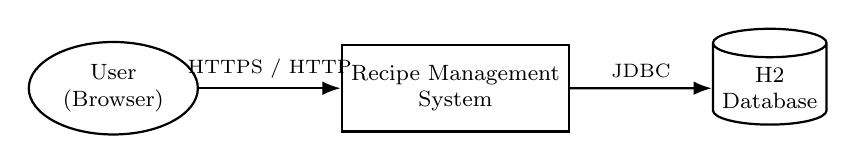
\begin{tikzpicture}[
  font=\footnotesize,
  comp/.style={draw, thick, minimum width=2.8cm, minimum height=1.1cm, align=center},
  actor/.style={draw, thick, ellipse, minimum width=1.6cm, align=center},
  data/.style={draw, thick, cylinder, shape border rotate=90, aspect=0.25, minimum height=1.2cm, align=center},
]
\node[actor] (user) {User\\(Browser)};
\node[comp, right=1.8cm of user] (app) {Recipe Management\\System};
\node[data, right=1.8cm of app] (db) {H2\\Database};

\draw[-{Latex}, thick] (user) -- node[above, font=\scriptsize]{HTTPS / HTTP} (app);
\draw[-{Latex}, thick] (app) -- node[above, font=\scriptsize]{JDBC} (db);
\end{tikzpicture}
\caption{System context: browser client, Javalin server, in-memory H2}
\label{fig:system-context}
\end{figure}

\section{Client Application Architecture}
\label{sec:fe-arch}

\subsection{Technology Stack}
The frontend is built strictly with \textbf{Vanilla HTML, CSS, and JavaScript}---no SPA framework. Each domain feature is a separate HTML page with a companion script, following a \textbf{Multi-Page Application (MPA)} pattern.

\subsection{Module Layout}
Source files reside under \path|src/main/resources/public/frontend/|:
\begin{verbatim}
frontend/
  login/         # Authentication entry point
  register/      # User creation
  recipe/        # Primary dashboard and recipe CRUD
  ingredients/   # Admin-only ingredient management
\end{verbatim}

\subsection{Runtime and Deployment}
\begin{itemize}[noitemsep]
  \item \textbf{Base URL:} \url{http://localhost:8081/} serves both the REST API and static assets.
  \item \textbf{Test isolation:} Do not run automated Selenium tests concurrently with a manual backend instance on the same port.
  \item \textbf{Presentation:} CSS is optional; markup must expose the DOM element IDs specified in Section~\ref{sec:ui-spec}.
\end{itemize}

\subsection{Client-Side State Model}
Ephemeral session state is stored in \texttt{sessionStorage}:
\begin{table}[htbp]
\centering
\footnotesize
\begin{tabular}{@{}llp{6.8cm}@{}}
\toprule
\textbf{Key} & \textbf{Type} & \textbf{Purpose} \\
\midrule
\texttt{auth-token} & string & Bearer token (JWT/UUID) from successful login \\
\texttt{is-admin} & string (\texttt{"true"}/\texttt{"false"}) & RBAC flag; controls visibility of admin navigation \\
\bottomrule
\end{tabular}
\caption{Browser session storage contract}
\label{tab:session-storage}
\end{table}

\subsection{API Client Integration (Fetch API)}
All network I/O uses the native \textbf{Fetch API}:
\begin{itemize}[noitemsep]
  \item JSON requests set \texttt{Content-Type: application/json}.
  \item Protected calls include \texttt{Authorization: Bearer <auth-token>}.
  \item Flow control checks \texttt{response.ok} and explicit status codes (\texttt{201}, \texttt{409}, \texttt{404}, etc.).
  \item CORS preflight is implicit; see Section~1.3.
\end{itemize}

\subsection{Navigation Map}
Figure~\ref{fig:nav-map} defines allowable page transitions. Unauthenticated users access \texttt{register} and \texttt{login}; authenticated users land on \texttt{recipe}; admins may navigate to \texttt{ingredients}.

\begin{figure}[htbp]
\centering
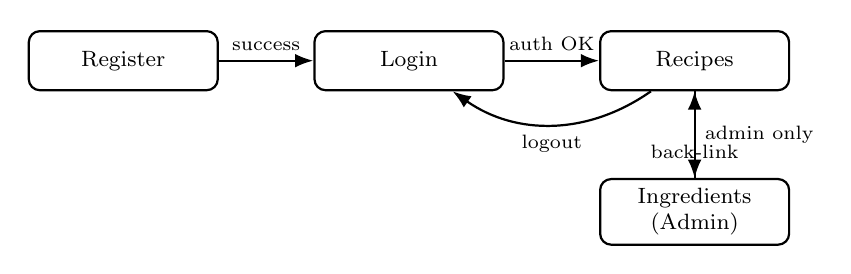
\begin{tikzpicture}[
  font=\footnotesize,
  page/.style={draw, thick, rounded corners, minimum width=2.4cm, minimum height=0.75cm, align=center},
  >=Latex,
]
\node[page] (reg) {Register};
\node[page, right=1.2cm of reg] (login) {Login};
\node[page, right=1.2cm of login] (recipe) {Recipes};
\node[page, below=1.1cm of recipe] (ing) {Ingredients\\(Admin)};

\draw[->, thick] (reg) -- node[above, font=\scriptsize]{success} (login);
\draw[->, thick] (login) -- node[above, font=\scriptsize]{auth OK} (recipe);
\draw[->, thick] (recipe) -- node[right, font=\scriptsize]{admin only} (ing);
\draw[->, thick, dashed] (ing) -- node[below, font=\scriptsize]{back-link} (recipe);
\draw[->, thick, bend left=35] (recipe) to node[below, font=\scriptsize]{logout} (login);
\end{tikzpicture}
\caption{MPA navigation / screen-flow diagram}
\label{fig:nav-map}
\end{figure}

\newpage
\section{Functional Requirements: Use Case Model}
\label{sec:use-cases}

\subsection{Use Case Diagram}
Figure~\ref{fig:use-case} follows UML use-case notation: actors outside the system boundary; ovals denote use cases grouped by package.

\begin{figure}[htbp]
\centering
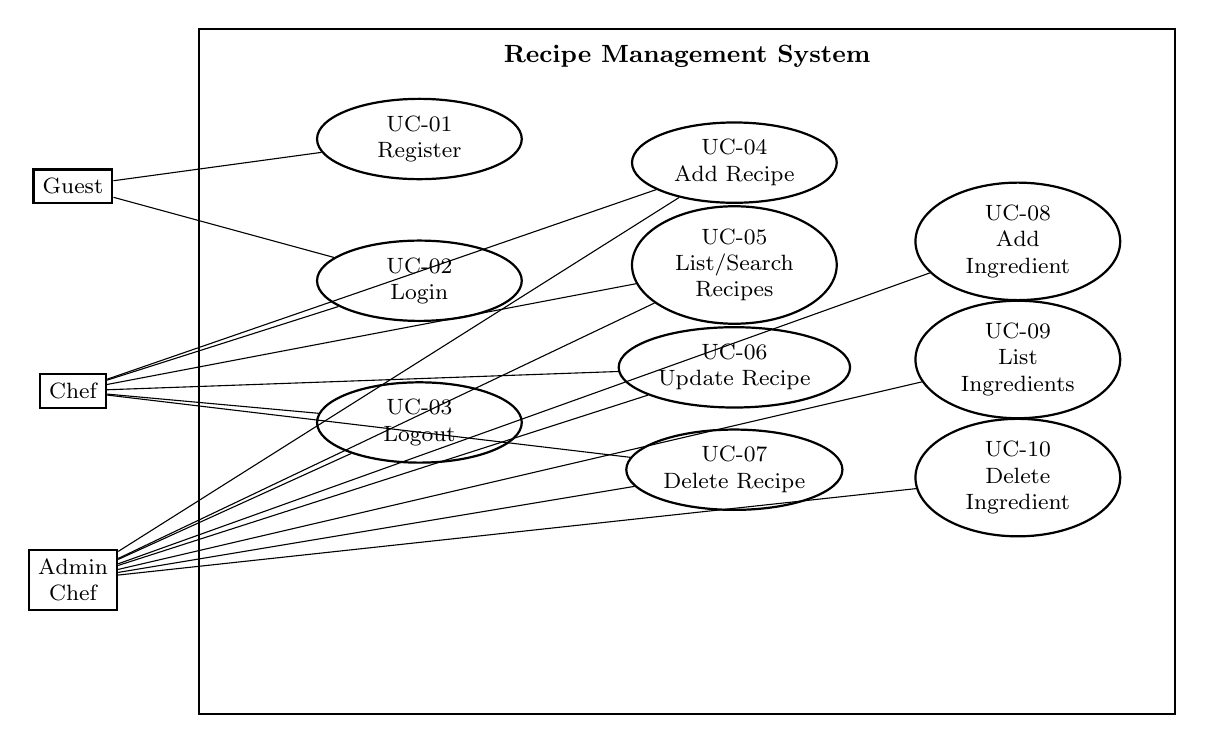
\begin{tikzpicture}[
  font=\footnotesize,
  usecase/.style={ellipse, draw, thick, minimum width=2.6cm, minimum height=0.85cm, align=center, inner sep=2pt},
  actor/.style={draw, thick, align=center},
  node distance=0.55cm and 0.35cm,
]
% System boundary
\draw[thick] (-0.6,-0.5) rectangle (11.8,8.2);
\node[font=\small\bfseries] at (5.6,7.85) {Recipe Management System};

% Actors
\node[actor] (guest) at (-2.2,6.2) {Guest};
\node[actor] (chef) at (-2.2,3.6) {Chef};
\node[actor] (admin) at (-2.2,1.2) {Admin\\Chef};

% Use cases
\node[usecase] (uc01) at (2.2,6.8) {UC-01\\Register};
\node[usecase] (uc02) at (2.2,5.0) {UC-02\\Login};
\node[usecase] (uc03) at (2.2,3.2) {UC-03\\Logout};

\node[usecase] (uc04) at (6.2,6.5) {UC-04\\Add Recipe};
\node[usecase] (uc05) at (6.2,5.2) {UC-05\\List/Search\\Recipes};
\node[usecase] (uc06) at (6.2,3.9) {UC-06\\Update Recipe};
\node[usecase] (uc07) at (6.2,2.6) {UC-07\\Delete Recipe};

\node[usecase] (uc08) at (9.8,5.5) {UC-08\\Add\\Ingredient};
\node[usecase] (uc09) at (9.8,4.0) {UC-09\\List\\Ingredients};
\node[usecase] (uc10) at (9.8,2.5) {UC-10\\Delete\\Ingredient};

% Associations
\draw (guest) -- (uc01); \draw (guest) -- (uc02);
\draw (chef) -- (uc02); \draw (chef) -- (uc03);
\foreach \uc in {uc04,uc05,uc06,uc07} \draw (chef) -- (\uc);
\draw (admin) -- (uc03);
\foreach \uc in {uc04,uc05,uc06,uc07,uc08,uc09,uc10} \draw (admin) -- (\uc);
\end{tikzpicture}
\caption{UML use case diagram (client-visible functionality)}
\label{fig:use-case}
\end{figure}

\subsection{Use Case Catalogue}
\begin{table}[htbp]
\centering
\footnotesize
\begin{tabular}{@{}cllp{4.2cm}@{}}
\toprule
\textbf{ID} & \textbf{Name} & \textbf{Primary Actor} & \textbf{Maps to README} \\
\midrule
UC-01 & Register Account & Guest & User Registration \\
UC-02 & Authenticate & Guest/Chef & User Login \\
UC-03 & Log Out & Chef & Logout (recipe page) \\
UC-04 & Add Recipe & Chef & Recipe Management \\
UC-05 & List/Search Recipes & Chef & Recipe Management \\
UC-06 & Update Recipe & Chef & Recipe Management \\
UC-07 & Delete Recipe & Chef & Recipe Management \\
UC-08 & Add Ingredient & Admin Chef & Ingredient Management \\
UC-09 & List Ingredients & Admin Chef & Ingredient Management \\
UC-10 & Delete Ingredient & Admin Chef & Ingredient Management \\
\bottomrule
\end{tabular}
\caption{Use case traceability to project requirements}
\label{tab:uc-catalogue}
\end{table}

\subsection{Use Case Specifications}
The following narratives follow the standard UML use-case specification template (brief description, pre/postconditions, basic and alternative flows).

\subsubsection{UC-01: Register Account}
\textbf{Location:} \path|frontend/register/| (\texttt{register-page.html}, \texttt{register-page.js}).

\textbf{Preconditions:} Guest is on the registration page.

\textbf{Basic Flow:}
\begin{enumerate}[label=\arabic*., leftmargin=*]
  \item Guest enters \texttt{username}, \texttt{email}, \texttt{password}, and \texttt{repeat password}.
  \item Guest clicks \texttt{register-button}.
  \item System validates all fields are non-empty and passwords match.
  \item System sends \texttt{POST} \path|/register| with JSON body \texttt{\{username, email, password\}}.
  \item System receives \texttt{201 Created} and redirects to the login page.
\end{enumerate}

\textbf{Alternative Flows:}
\begin{itemize}[noitemsep]
  \item \textbf{3a} Validation fails $\rightarrow$ display alert; remain on page.
  \item \textbf{5a} \texttt{409 Conflict} $\rightarrow$ alert duplicate user/email.
  \item \textbf{5b} Other error or network failure $\rightarrow$ alert generic or network error.
\end{itemize}

\subsubsection{UC-02: Authenticate}
\textbf{Location:} \path|frontend/login/|.

\textbf{Basic Flow:}
\begin{enumerate}[label=\arabic*., leftmargin=*]
  \item Guest enters \texttt{username} and \texttt{password}; clicks \texttt{login-button}.
  \item System sends \texttt{POST} \path|/login| with JSON credentials.
  \item On \texttt{200 OK}, system parses token and admin flag (JSON \texttt{\{token, isAdmin\}} or plaintext \texttt{"<token> <isAdmin>"}).
  \item System stores \texttt{auth-token} and \texttt{is-admin} in \texttt{sessionStorage}.
  \item System redirects to \path|frontend/recipe/recipe-page.html|.
\end{enumerate}

\textbf{Alternative Flows:} \texttt{401} $\rightarrow$ alert invalid credentials; empty fields $\rightarrow$ alert before request.

\subsubsection{UC-03: Log Out}
\textbf{Location:} \path|frontend/recipe/recipe-page.js| (\texttt{processLogout}).

\textbf{Basic Flow:}
\begin{enumerate}[label=\arabic*., leftmargin=*]
  \item Chef clicks \texttt{logout-button} (visible when \texttt{auth-token} exists).
  \item System sends \texttt{POST} \path|/logout| with Bearer token.
  \item On \texttt{200 OK}, system clears \texttt{sessionStorage} and redirects to login.
\end{enumerate}

\subsubsection{UC-04 through UC-07: Recipe CRUD}
\textbf{Location:} \path|frontend/recipe/|. All flows require a valid Bearer token. After mutating operations, the client refreshes the in-memory \texttt{recipes} array and re-renders \texttt{recipe-list}.

\textbf{Name-to-ID resolution (client pattern):} Update and delete forms accept a \textbf{recipe name}. The client resolves the REST path parameter by case-insensitive match against the locally cached list from \texttt{GET /recipes}, then calls \texttt{PUT /recipes/\{id\}} or \texttt{DELETE /recipes/\{id\}}. If no match exists, alert ``Recipe not found in list!''

\begin{table}[htbp]
\centering
\footnotesize
\begin{tabular}{@{}llll@{}}
\toprule
\textbf{UC} & \textbf{UI Trigger} & \textbf{HTTP} & \textbf{Success} \\
\midrule
UC-04 & \texttt{add-recipe-submit-input} & \texttt{POST /recipes} & \texttt{201}, refresh list \\
UC-05 & page load / \texttt{search-button} & \texttt{GET /recipes} or \texttt{?name=} & \texttt{200}/\texttt{404} $\rightarrow$ render \\
UC-06 & \texttt{update-recipe-submit-input} & \texttt{PUT /recipes/\{id\}} & \texttt{200}, refresh \\
UC-07 & \texttt{delete-recipe-submit-input} & \texttt{DELETE /recipes/\{id\}} & \texttt{200}, refresh \\
\bottomrule
\end{tabular}
\caption{Recipe use cases and REST mapping}
\label{tab:recipe-uc}
\end{table}

\subsubsection{UC-08 through UC-10: Ingredient Management (Admin)}
\textbf{Location:} \path|frontend/ingredients/|. Accessible when \texttt{sessionStorage.is-admin === "true"}. Delete resolves ingredient \textbf{name} to \texttt{id} via local cache (same pattern as recipes). Successful delete accepts \texttt{204 No Content} or \texttt{200 OK}.

\newpage
\section{User Interface Specifications}
\label{sec:ui-spec}

Each subsection lists mandatory DOM identifiers (wireframe-level specification per ISO/IEC/IEEE 29148 Section~8) and required JavaScript behaviors.

\subsection{Registration Page}
\begin{table}[htbp]
\centering
\footnotesize
\begin{tabular}{@{}lll@{}}
\toprule
\textbf{Element ID} & \textbf{Control} & \textbf{Requirement} \\
\midrule
\texttt{username-input} & text & Required; sent to API \\
\texttt{email-input} & email & Required; sent to API \\
\texttt{password-input} & password & Required; sent to API \\
\texttt{repeat-password-input} & password & Client-only confirmation \\
\texttt{register-button} & button & Invokes \texttt{processRegistration()} \\
\bottomrule
\end{tabular}
\caption{Registration page UI inventory}
\end{table}

\subsection{Login Page}
\begin{table}[htbp]
\centering
\footnotesize
\begin{tabular}{@{}lll@{}}
\toprule
\textbf{Element ID} & \textbf{Control} & \textbf{Requirement} \\
\midrule
\texttt{login-input} & text & Username for \texttt{POST /login} \\
\texttt{password-input} & password & Password for \texttt{POST /login} \\
\texttt{login-button} & button & Invokes \texttt{processLogin()} \\
\texttt{logout-button} & button & Hidden by default; optional testing aid \\
\bottomrule
\end{tabular}
\caption{Login page UI inventory}
\end{table}

\subsection{Recipe Dashboard}
\begin{table}[htbp]
\centering
\footnotesize
\begin{tabular}{@{}llp{5.5cm}@{}}
\toprule
\textbf{Element ID} & \textbf{Control} & \textbf{Requirement} \\
\midrule
\texttt{admin-link} & anchor & Hidden initially; shown when \texttt{is-admin} is \texttt{"true"}; links to ingredients page \\
\texttt{logout-button} & button & Hidden until \texttt{auth-token} present \\
\texttt{search-input}, \texttt{search-button} & text, button & Invokes \texttt{searchRecipes()} \\
\texttt{recipe-list} & \texttt{<ul>} & Populated by \texttt{refreshRecipeList()} \\
\texttt{add-recipe-name-input} & text & Add form \\
\texttt{add-recipe-instructions-input} & textarea & Add form \\
\texttt{add-recipe-submit-input} & button & Invokes \texttt{addRecipe()} \\
\texttt{update-recipe-name-input} & text & Name lookup for update \\
\texttt{update-recipe-instructions-input} & textarea & New instructions \\
\texttt{update-recipe-submit-input} & button & Invokes \texttt{updateRecipe()} \\
\texttt{delete-recipe-name-input} & text & Name lookup for delete \\
\texttt{delete-recipe-submit-input} & button & Invokes \texttt{deleteRecipe()} \\
\bottomrule
\end{tabular}
\caption{Recipe page UI inventory}
\end{table}

\textbf{Page-load behavior:} On \texttt{DOMContentLoaded}, call \texttt{getRecipes()}, show \texttt{admin-link} via admin check (equivalent to \texttt{displayAdminLink()}), wire event handlers, and conditionally display \texttt{logout-button}.

\textbf{Required functions:} \texttt{getRecipes()}, \texttt{refreshRecipeList()}, \texttt{addRecipe()}, \texttt{updateRecipe()}, \texttt{deleteRecipe()}, \texttt{searchRecipes()}, \texttt{processLogout()}.

\subsection{Ingredient Management Page (Admin)}
\begin{table}[htbp]
\centering
\footnotesize
\begin{tabular}{@{}lll@{}}
\toprule
\textbf{Element ID} & \textbf{Control} & \textbf{Requirement} \\
\midrule
\texttt{back-link} & anchor & Return to recipe dashboard \\
\texttt{ingredient-list} & \texttt{<ul>} & Rendered by \texttt{refreshIngredientList()} \\
\texttt{add-ingredient-name-input} & text & Add form \\
\texttt{add-ingredient-submit-button} & button & Invokes \texttt{addIngredient()} \\
\texttt{delete-ingredient-name-input} & text & Name lookup for delete \\
\texttt{delete-ingredient-submit-button} & button & Invokes \texttt{deleteIngredient()} \\
\bottomrule
\end{tabular}
\caption{Ingredient page UI inventory}
\end{table}

\textbf{Page-load behavior:} Call \texttt{getIngredients()}. Verify \texttt{auth-token} and admin status via \texttt{sessionStorage} before allowing mutations.

\textbf{Required functions:} \texttt{getIngredients()}, \texttt{addIngredient()}, \texttt{deleteIngredient()}, \texttt{refreshIngredientList()}.

\section{Client--Server Interaction Models}
\label{sec:interaction}

\subsection{Sequence Diagram: User Registration}
Figure~\ref{fig:seq-register} models UC-01 as a UML interaction diagram.

\begin{figure}[htbp]
\centering
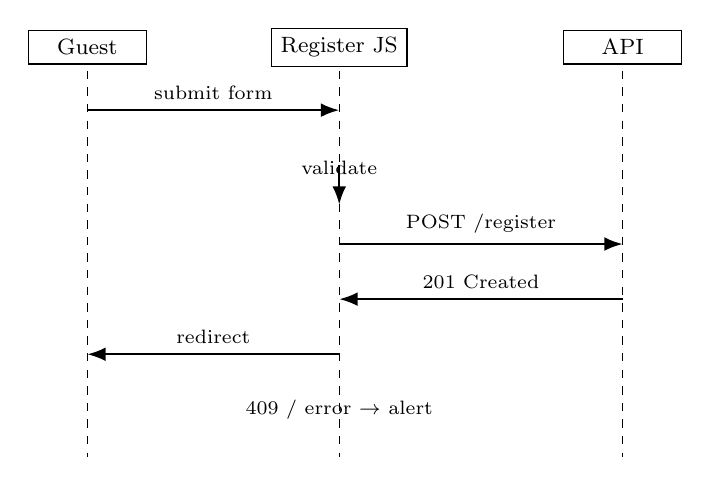
\begin{tikzpicture}[
  font=\footnotesize,
  actor/.style={rectangle, draw, minimum width=1.5cm},
  lifeline/.style={dashed},
  msg/.style={-{Latex}, thick},
]
\node[actor] (user) at (0,0) {Guest};
\node[actor] (page) at (3.2,0) {Register JS};
\node[actor] (api) at (6.8,0) {API};

\foreach \x in {0,3.2,6.8} \draw[dashed] (\x,-0.3) -- (\x,-5.2);

\draw[msg] (0,-0.8) -- node[above, font=\scriptsize]{submit form} (3.2,-0.8);
\draw[msg] (3.2,-1.5) -- node[above, font=\scriptsize]{validate} (3.2,-2.0);
\draw[msg] (3.2,-2.5) -- node[above, font=\scriptsize]{POST /register} (6.8,-2.5);
\draw[msg] (6.8,-3.2) -- node[above, font=\scriptsize]{201 Created} (3.2,-3.2);
\draw[msg] (3.2,-3.9) -- node[above, font=\scriptsize]{redirect} (0,-3.9);
\node[font=\scriptsize] at (3.2,-4.6) {409 / error $\rightarrow$ alert};
\end{tikzpicture}
\caption{Sequence diagram: registration (UC-01)}
\label{fig:seq-register}
\end{figure}

\subsection{Sequence Diagram: Login and Session Establishment}
\begin{figure}[htbp]
\centering
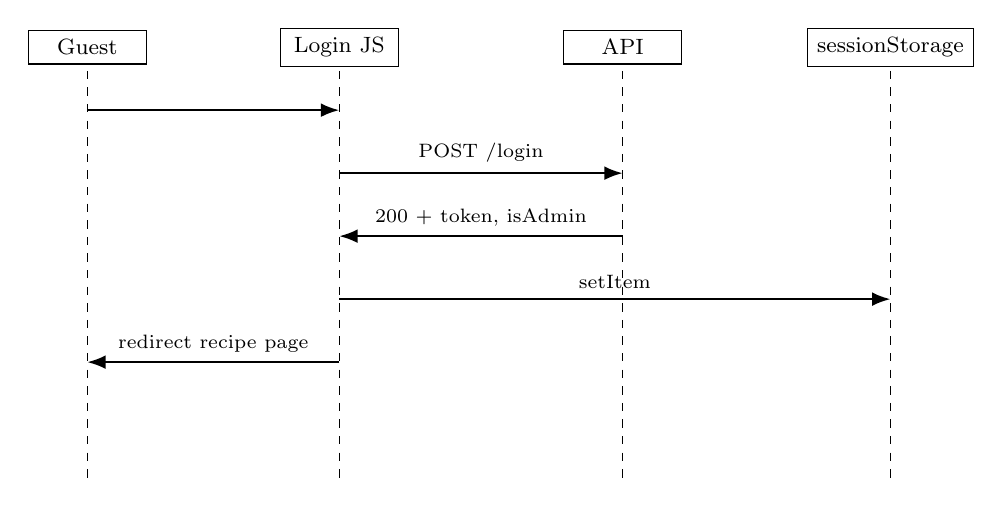
\begin{tikzpicture}[
  font=\footnotesize,
  actor/.style={rectangle, draw, minimum width=1.5cm},
  msg/.style={-{Latex}, thick},
]
\node[actor] (user) at (0,0) {Guest};
\node[actor] (page) at (3.2,0) {Login JS};
\node[actor] (api) at (6.8,0) {API};
\node[actor] (store) at (10.2,0) {sessionStorage};

\foreach \x in {0,3.2,6.8,10.2} \draw[dashed] (\x,-0.3) -- (\x,-5.5);

\draw[thick,-{Latex}] (0,-0.8) -- (3.2,-0.8);
\draw[thick,-{Latex}] (3.2,-1.6) -- node[above, font=\scriptsize]{POST /login} (6.8,-1.6);
\draw[thick,-{Latex}] (6.8,-2.4) -- node[above, font=\scriptsize]{200 + token, isAdmin} (3.2,-2.4);
\draw[thick,-{Latex}] (3.2,-3.2) -- node[above, font=\scriptsize]{setItem} (10.2,-3.2);
\draw[thick,-{Latex}] (3.2,-4.0) -- node[above, font=\scriptsize]{redirect recipe page} (0,-4.0);
\end{tikzpicture}
\caption{Sequence diagram: authentication (UC-02)}
\label{fig:seq-login}
\end{figure}

\subsection{Activity Diagram: Update Recipe by Name}
The client resolves the REST identifier before invoking the API (UML activity semantics):

\begin{enumerate}[label=\arabic*., leftmargin=*]
  \item Read \texttt{update-recipe-name-input} and \texttt{update-recipe-instructions-input}.
  \item If either empty $\rightarrow$ alert and stop.
  \item Search \texttt{recipes[]} for case-insensitive name match.
  \item If not found $\rightarrow$ alert and stop.
  \item \texttt{PUT /recipes/\{id\}} with updated \texttt{instructions}; on \texttt{200} refresh list.
\end{enumerate}

\section{Non-Functional Requirements (Client)}
\begin{itemize}[noitemsep]
  \item \textbf{Usability:} Use browser \texttt{alert()} for validation and error feedback unless otherwise specified.
  \item \textbf{Security:} No credentials persisted beyond \texttt{sessionStorage}; protected pages must attach Bearer tokens.
  \item \textbf{Compatibility:} Modern browsers with Fetch and \texttt{sessionStorage} support.
  \item \textbf{Maintainability:} One HTML/JS pair per feature directory; shared \texttt{BASE\_URL = "http://localhost:8081"}.
\end{itemize}

\section{External References}
\begin{itemize}[noitemsep]
  \item MDN Fetch API: \url{https://developer.mozilla.org/en-US/docs/Web/API/Fetch_API/Using_Fetch}
  \item MDN CORS: \url{https://developer.mozilla.org/en-US/docs/Web/HTTP/CORS}
  \item ISO/IEC/IEEE 29148:2018 --- Systems and software engineering --- Life cycle processes --- Requirements engineering
\end{itemize}

\end{document}